%\documentclass[letterpaper,10pt,titlepage]{article}
\documentclass[onecolumn]{IEEEtran}

\usepackage{graphicx}                                        
\usepackage{amssymb}                                         
\usepackage{amsmath}                                         
\usepackage{amsthm}                                          

\usepackage{alltt}
\usepackage{float}
\usepackage{color}
\usepackage{url}

\usepackage{balance}
\usepackage[TABBOTCAP, tight]{subfigure}
\usepackage{enumitem}
\usepackage{pstricks, pst-node}
%don't really worry about what this does, if it doesn't immediately make sense to you.
%just have it ready for use, and then ignore it.
\usepackage{fancyvrb}
\usepackage{color}
\usepackage[latin1]{inputenc}


\makeatletter
\def\PY@reset{\let\PY@it=\relax \let\PY@bf=\relax%
    \let\PY@ul=\relax \let\PY@tc=\relax%
    \let\PY@bc=\relax \let\PY@ff=\relax}
\def\PY@tok#1{\csname PY@tok@#1\endcsname}
\def\PY@toks#1+{\ifx\relax#1\empty\else%
    \PY@tok{#1}\expandafter\PY@toks\fi}
\def\PY@do#1{\PY@bc{\PY@tc{\PY@ul{%
    \PY@it{\PY@bf{\PY@ff{#1}}}}}}}
\def\PY#1#2{\PY@reset\PY@toks#1+\relax+\PY@do{#2}}

\expandafter\def\csname PY@tok@gd\endcsname{\def\PY@tc##1{\textcolor[rgb]{0.63,0.00,0.00}{##1}}}
\expandafter\def\csname PY@tok@gu\endcsname{\let\PY@bf=\textbf\def\PY@tc##1{\textcolor[rgb]{0.50,0.00,0.50}{##1}}}
\expandafter\def\csname PY@tok@gt\endcsname{\def\PY@tc##1{\textcolor[rgb]{0.00,0.25,0.82}{##1}}}
\expandafter\def\csname PY@tok@gs\endcsname{\let\PY@bf=\textbf}
\expandafter\def\csname PY@tok@gr\endcsname{\def\PY@tc##1{\textcolor[rgb]{1.00,0.00,0.00}{##1}}}
\expandafter\def\csname PY@tok@cm\endcsname{\let\PY@it=\textit\def\PY@tc##1{\textcolor[rgb]{0.25,0.50,0.50}{##1}}}
\expandafter\def\csname PY@tok@vg\endcsname{\def\PY@tc##1{\textcolor[rgb]{0.10,0.09,0.49}{##1}}}
\expandafter\def\csname PY@tok@m\endcsname{\def\PY@tc##1{\textcolor[rgb]{0.40,0.40,0.40}{##1}}}
\expandafter\def\csname PY@tok@mh\endcsname{\def\PY@tc##1{\textcolor[rgb]{0.40,0.40,0.40}{##1}}}
\expandafter\def\csname PY@tok@go\endcsname{\def\PY@tc##1{\textcolor[rgb]{0.50,0.50,0.50}{##1}}}
\expandafter\def\csname PY@tok@ge\endcsname{\let\PY@it=\textit}
\expandafter\def\csname PY@tok@vc\endcsname{\def\PY@tc##1{\textcolor[rgb]{0.10,0.09,0.49}{##1}}}
\expandafter\def\csname PY@tok@il\endcsname{\def\PY@tc##1{\textcolor[rgb]{0.40,0.40,0.40}{##1}}}
\expandafter\def\csname PY@tok@cs\endcsname{\let\PY@it=\textit\def\PY@tc##1{\textcolor[rgb]{0.25,0.50,0.50}{##1}}}
\expandafter\def\csname PY@tok@cp\endcsname{\def\PY@tc##1{\textcolor[rgb]{0.74,0.48,0.00}{##1}}}
\expandafter\def\csname PY@tok@gi\endcsname{\def\PY@tc##1{\textcolor[rgb]{0.00,0.63,0.00}{##1}}}
\expandafter\def\csname PY@tok@gh\endcsname{\let\PY@bf=\textbf\def\PY@tc##1{\textcolor[rgb]{0.00,0.00,0.50}{##1}}}
\expandafter\def\csname PY@tok@ni\endcsname{\let\PY@bf=\textbf\def\PY@tc##1{\textcolor[rgb]{0.60,0.60,0.60}{##1}}}
\expandafter\def\csname PY@tok@nl\endcsname{\def\PY@tc##1{\textcolor[rgb]{0.63,0.63,0.00}{##1}}}
\expandafter\def\csname PY@tok@nn\endcsname{\let\PY@bf=\textbf\def\PY@tc##1{\textcolor[rgb]{0.00,0.00,1.00}{##1}}}
\expandafter\def\csname PY@tok@no\endcsname{\def\PY@tc##1{\textcolor[rgb]{0.53,0.00,0.00}{##1}}}
\expandafter\def\csname PY@tok@na\endcsname{\def\PY@tc##1{\textcolor[rgb]{0.49,0.56,0.16}{##1}}}
\expandafter\def\csname PY@tok@nb\endcsname{\def\PY@tc##1{\textcolor[rgb]{0.00,0.50,0.00}{##1}}}
\expandafter\def\csname PY@tok@nc\endcsname{\let\PY@bf=\textbf\def\PY@tc##1{\textcolor[rgb]{0.00,0.00,1.00}{##1}}}
\expandafter\def\csname PY@tok@nd\endcsname{\def\PY@tc##1{\textcolor[rgb]{0.67,0.13,1.00}{##1}}}
\expandafter\def\csname PY@tok@ne\endcsname{\let\PY@bf=\textbf\def\PY@tc##1{\textcolor[rgb]{0.82,0.25,0.23}{##1}}}
\expandafter\def\csname PY@tok@nf\endcsname{\def\PY@tc##1{\textcolor[rgb]{0.00,0.00,1.00}{##1}}}
\expandafter\def\csname PY@tok@si\endcsname{\let\PY@bf=\textbf\def\PY@tc##1{\textcolor[rgb]{0.73,0.40,0.53}{##1}}}
\expandafter\def\csname PY@tok@s2\endcsname{\def\PY@tc##1{\textcolor[rgb]{0.73,0.13,0.13}{##1}}}
\expandafter\def\csname PY@tok@vi\endcsname{\def\PY@tc##1{\textcolor[rgb]{0.10,0.09,0.49}{##1}}}
\expandafter\def\csname PY@tok@nt\endcsname{\let\PY@bf=\textbf\def\PY@tc##1{\textcolor[rgb]{0.00,0.50,0.00}{##1}}}
\expandafter\def\csname PY@tok@nv\endcsname{\def\PY@tc##1{\textcolor[rgb]{0.10,0.09,0.49}{##1}}}
\expandafter\def\csname PY@tok@s1\endcsname{\def\PY@tc##1{\textcolor[rgb]{0.73,0.13,0.13}{##1}}}
\expandafter\def\csname PY@tok@sh\endcsname{\def\PY@tc##1{\textcolor[rgb]{0.73,0.13,0.13}{##1}}}
\expandafter\def\csname PY@tok@sc\endcsname{\def\PY@tc##1{\textcolor[rgb]{0.73,0.13,0.13}{##1}}}
\expandafter\def\csname PY@tok@sx\endcsname{\def\PY@tc##1{\textcolor[rgb]{0.00,0.50,0.00}{##1}}}
\expandafter\def\csname PY@tok@bp\endcsname{\def\PY@tc##1{\textcolor[rgb]{0.00,0.50,0.00}{##1}}}
\expandafter\def\csname PY@tok@c1\endcsname{\let\PY@it=\textit\def\PY@tc##1{\textcolor[rgb]{0.25,0.50,0.50}{##1}}}
\expandafter\def\csname PY@tok@kc\endcsname{\let\PY@bf=\textbf\def\PY@tc##1{\textcolor[rgb]{0.00,0.50,0.00}{##1}}}
\expandafter\def\csname PY@tok@c\endcsname{\let\PY@it=\textit\def\PY@tc##1{\textcolor[rgb]{0.25,0.50,0.50}{##1}}}
\expandafter\def\csname PY@tok@mf\endcsname{\def\PY@tc##1{\textcolor[rgb]{0.40,0.40,0.40}{##1}}}
\expandafter\def\csname PY@tok@err\endcsname{\def\PY@bc##1{\setlength{\fboxsep}{0pt}\fcolorbox[rgb]{1.00,0.00,0.00}{1,1,1}{\strut ##1}}}
\expandafter\def\csname PY@tok@kd\endcsname{\let\PY@bf=\textbf\def\PY@tc##1{\textcolor[rgb]{0.00,0.50,0.00}{##1}}}
\expandafter\def\csname PY@tok@ss\endcsname{\def\PY@tc##1{\textcolor[rgb]{0.10,0.09,0.49}{##1}}}
\expandafter\def\csname PY@tok@sr\endcsname{\def\PY@tc##1{\textcolor[rgb]{0.73,0.40,0.53}{##1}}}
\expandafter\def\csname PY@tok@mo\endcsname{\def\PY@tc##1{\textcolor[rgb]{0.40,0.40,0.40}{##1}}}
\expandafter\def\csname PY@tok@kn\endcsname{\let\PY@bf=\textbf\def\PY@tc##1{\textcolor[rgb]{0.00,0.50,0.00}{##1}}}
\expandafter\def\csname PY@tok@mi\endcsname{\def\PY@tc##1{\textcolor[rgb]{0.40,0.40,0.40}{##1}}}
\expandafter\def\csname PY@tok@gp\endcsname{\let\PY@bf=\textbf\def\PY@tc##1{\textcolor[rgb]{0.00,0.00,0.50}{##1}}}
\expandafter\def\csname PY@tok@o\endcsname{\def\PY@tc##1{\textcolor[rgb]{0.40,0.40,0.40}{##1}}}
\expandafter\def\csname PY@tok@kr\endcsname{\let\PY@bf=\textbf\def\PY@tc##1{\textcolor[rgb]{0.00,0.50,0.00}{##1}}}
\expandafter\def\csname PY@tok@s\endcsname{\def\PY@tc##1{\textcolor[rgb]{0.73,0.13,0.13}{##1}}}
\expandafter\def\csname PY@tok@kp\endcsname{\def\PY@tc##1{\textcolor[rgb]{0.00,0.50,0.00}{##1}}}
\expandafter\def\csname PY@tok@w\endcsname{\def\PY@tc##1{\textcolor[rgb]{0.73,0.73,0.73}{##1}}}
\expandafter\def\csname PY@tok@kt\endcsname{\def\PY@tc##1{\textcolor[rgb]{0.69,0.00,0.25}{##1}}}
\expandafter\def\csname PY@tok@ow\endcsname{\let\PY@bf=\textbf\def\PY@tc##1{\textcolor[rgb]{0.67,0.13,1.00}{##1}}}
\expandafter\def\csname PY@tok@sb\endcsname{\def\PY@tc##1{\textcolor[rgb]{0.73,0.13,0.13}{##1}}}
\expandafter\def\csname PY@tok@k\endcsname{\let\PY@bf=\textbf\def\PY@tc##1{\textcolor[rgb]{0.00,0.50,0.00}{##1}}}
\expandafter\def\csname PY@tok@se\endcsname{\let\PY@bf=\textbf\def\PY@tc##1{\textcolor[rgb]{0.73,0.40,0.13}{##1}}}
\expandafter\def\csname PY@tok@sd\endcsname{\let\PY@it=\textit\def\PY@tc##1{\textcolor[rgb]{0.73,0.13,0.13}{##1}}}

\def\PYZbs{\char`\\}
\def\PYZus{\char`\_}
\def\PYZob{\char`\{}
\def\PYZcb{\char`\}}
\def\PYZca{\char`\^}
\def\PYZam{\char`\&}
\def\PYZlt{\char`\<}
\def\PYZgt{\char`\>}
\def\PYZsh{\char`\#}
\def\PYZpc{\char`\%}
\def\PYZdl{\char`\$}
\def\PYZti{\char`\~}
% for compatibility with earlier versions
\def\PYZat{@}
\def\PYZlb{[}
\def\PYZrb{]}
\makeatother


\usepackage{geometry}
\geometry{textheight=8.5in, textwidth=6in, margin=0.75in}

%random comment

\newcommand{\cred}[1]{{\color{red}#1}}
\newcommand{\cblue}[1]{{\color{blue}#1}}

%% This is supposed to make the 'references' part show up in the TOC
\usepackage[nottoc,numbib]{tocbibind}
\usepackage{titling}
\usepackage{blindtext}
\usepackage{graphicx}
\graphicspath{ {images/} }

\usepackage{hyperref}
\usepackage{geometry}

\def\name{David Winkler}

%% The following metadata will show up in the PDF properties
\hypersetup{
  colorlinks = true,
  urlcolor = blue,
  citecolor = black,
  linkcolor = black,	% MY ADDITION
  pdfauthor = {\name},
  pdfkeywords = {CS462 angularjs webdev research},
  pdftitle = {CS 462 Midterm Progress Report},
  pdfsubject = {CS 462 Midterm Progress Report},
  pdfpagemode = UseNone
}

\title{February Progress Report}
\author{David Winkler \and Christopher Nguyen \and Benny Zhao}
\date{12 Feb. 2016}

\begin{document}

%%%%%%%%%%%%%%%%%%%%%%%%%%%%%%%%%%%%%%%%%%%%%%%%%%%%%%%%%
%%%%% TITLE PAGE
%%%%%%%%%%%%%%%%%%%%%%%%%%%%%%%%%%%%%%%%%%%%%%%%%%%%%%%%%
% Title sourced from http://www.latextemplates.com/template/university-assignment-title-page
\begin{titlepage}
	\newcommand{\HRule}{\rule{\linewidth}{0.5mm}} % Defines a new command for the horizontal lines, change thickness here
	\center % Center everything on the page
    
    \begin{figure}
        \centering
        
\includegraphics[width=0.8\textwidth]{ctr_logo.png}
    \end{figure}
 
	\textsc{\LARGE Oregon State University}\\[1.5cm] % Name of university
	\textsc{\Large CS462 - Winter 2016}\\[0.5cm] % Major heading such as course name
	\textsc{\large Senior Design Project II}\\[0.5cm] % Minor heading such as course title

	{\large 12 February 2016}\\[1cm]
    
	\HRule \\[0.4cm]
		{ \huge \bfseries Midterm Progress Report}\\[0.4cm] % Title of document
	\HRule \\[1.5cm]

	\begin{minipage}{0.4\textwidth}
		\begin{flushleft} \large
			\emph{Authors:}\\
			David \textsc{Winkler}\\ % Name
			Chris \textsc{Nguyen}\\
			Benny \textsc{Zhao}
		\end{flushleft}
	\end{minipage}
	~
	\begin{minipage}{0.4\textwidth}
		\begin{flushright} \large
			\emph{Instructor:} \\
			D. Kevin \textsc{McGrath} \\
            \emph{TA:} \\
            John \textsc{Dodge}
		\end{flushright}
	\end{minipage}\\[2cm]
    
    \begin{minipage}{1.0\textwidth}
        \begin{abstract}
            This document serves to describe the history and current state of our project. We attempt to give the final goal of our application, and the step we have taken to implement it. We describe how we implemented the features, and why we made the decisions we did. We list the features that are not yet implemented, and how we plan to implement them. We will demonstrate our application using screenshots and provide code examples to illustrate our designs. We will also describe our clients' reactions to our work thus far.        
        \end{abstract}
    \end{minipage}

\end{titlepage}

%%%%%%%%%%%%%%%%%%%%%%%%%%%%%%%%%%%%%%%%%%%%%%%%%%%%%%%%%%%%%%%%%%%%%%%%%%%%%%%%
%%%%% TOC
%%%%%%%%%%%%%%%%%%%%%%%%%%%%%%%%%%%%%%%%%%%%%%%%%%%%%%%%%%%%%%%%%%%%%%%%%%%%%%%%
\tableofcontents
%\vfill % Fill the rest of the page with whitespace
\pagebreak	% Keeps on separate pages

%%%%%%%%%%%%%%%%%%%%%%%%%%%%%%%%%%%%%%%%%%%%%%%%%%%%%%%%%%%%%%%%%%%%%%%%%%%%%%%%
%%%%% CONTEXT
%%%%%%%%%%%%%%%%%%%%%%%%%%%%%%%%%%%%%%%%%%%%%%%%%%%%%%%%%%%%%%%%%%%%%%%%%%%%%%%%
\section{Project Context}
Research scientists spend a lot of time finding information related to their research. They need to collaborate with other researchers to share their expertise, consult on difficult issues, and network. They also need to stay abreast of developments in their field so that they don't end up reinventing the wheel. And perhaps most importantly, they need to search for funding opportunities so that they can continue their research. With these considerations in mind, a team of research scientists at the Pacific Northwest National Laboratory has proposed a new web application, titled Connected to Research. 

Connected to Research is a web application that seeks to make life easier for research scientists. When complete, it will feature portals that allow users to trim some work that must be done before research can take place. Last year, a senior design team worked on the Publications component. The Publications component seeks to connect each user to published works that are relevant to the user's interests. This year, our team has been tackling the Funding component. The goal for the Funding component is analogous to that of the Publications component. It will remove the hassle of researching funding opportunities by connecting researchers to opportunities that apply to their areas of interest.

\subsection{Funding Sources}
Our clients gave us a short list of funding sources they wanted us to pull data from, but after a couple meetings, we decided that most of the data we needed would come from two sources: Grants.gov and FedBizOpps.gov. Grants.gov is a site managed by the US government that publishes all public grants from all federal agencies that award grants. FedBizOpps.gov is a site that publishes information about government procurement contracts. Both government agencies list a need for something and offer to buy it from businesses that apply. Both sites allow users to search through their databases, but until now, there has not been an easy way for researchers to find all funding opportunities related to their specific interests. 

\subsection{Requirements}
At the beginning, we separated our project into 3 major categories of work. The first category that needed to be completed was the one involving the database. Before we did anything, we needed to define the set of funding sources we would support. After meeting with our clients, we determined that the most effective selection would be to take information from FedBizOpps.gov and Grants.gov. With the combined data from both of these sources, we would get enough data to make our website functional. 

To implement this feature, our clients gave us a simple, open-ended set of requirements. We divided the requirements into three categories according to the order in which we thought they needed to be done. The following paragraphs are a description of our requirements. 

First, we need to define the sources of funding that will provide the data for our database. We need to define the information that they store to define the database tables. We need to define the database and a set of parsing scripts to fill them. We need to define how other Connected to Research components will need to interact with the funding component. We need to decide how best to parse information from the funding sources and write the scripts. Then we need to implement database accessor functions using the client's preferred language. 

Second, we need to work on the system for interacting with user interests. Our clients did not have many requests for this part, so the requirements are sparse. Essentially, we must have some mechanism mapping the funding opportunities to user interests. 

Third, we need a workable user interface. This may be the most important part because this project is still a proof-of-concept that will hopefully bloom into a fully-featured web application. We need to develop methods to display funding opportunities to the user, which will be done similar to the previous team's work. We will need to allow images embedded in the opportunity description. We will need to allow users to bookmark opportunities and display them in a chronological list. This will be important for users who need to be reminded of approaching deadlines. Otherwise, they would need to manually manage their own notification systems. Users will also need to 'dog-ear' opportunities separately from the bookmarks. This is for the case where researchers want to make one large sweep to find any opportunity that might apply to them, and then choose which to actually apply to through bookmarking. Users will also want to share opportunities with other users, a feature which will likely tie-in with the 'People' component of Connected to Research, where users can connect to other researchers through the web app. 


%%%%%%%%%%%%%%%%%%%%%%%%%%%%%%%%%%%%%%%%%%%%%%%%%%%%%%%%%%%%%%%%%%%%%%%%%%%%%%%%
%%%%% OUR WORK
%%%%%%%%%%%%%%%%%%%%%%%%%%%%%%%%%%%%%%%%%%%%%%%%%%%%%%%%%%%%%%%%%%%%%%%%%%%%%%%%
\section{Our Work So Far}
Because the previous team laid the foundation for our contributions to build on, much of our work involves understanding their codebase and adapting it to our changes. The main thrust of our efforts has been to develop a database for funding opportunities, and the scripts that fill them. Eventually, we contacted a member of the previous team, Anton Dovzhik, to help us configure the website properly. Afterwards, we focused on building our app starting with the database and parsers. 

We needed to investigate the metadata from our funding sources and determine the best way to take their data and put it into our database. We searched through the documentation for FedBizOpps and found that they published two types of files through an FTP portal on their website. They published a weekly XML file, which contained a well-formed XML document that lists all of the funding opportunities listed in their database. They also publish nightly files which they call XML, but which aren't actually XML. These nightly files contain the opportunities that have been added or updated since the last nightly file. They do not conform to any XML rules, and are more like formatted text documents. For Grants.gov, we found that they publish daily dumps of their entire grant database. These files are much more straightforward to parse. Their documentation is also accurate, unlike FedBizOpps. We parse these XML files using PHP and insert each valid record into our database. Our clients defined which types of records such be inserted into our database.  

\subsection{Grants.gov Parser}
One of the parsers is for the website Grants.gov. Grants.gov supplies an XML file that includes all of its current opportunities while FedBizOpps.gov supplies two types of files which are XML and formatted text that includes all of its current opportunities. We parse these files then use the parsed information to populate the database.  

For Grants.gov, the parser has three parts. The three parts consist of reading the XML file into a buffer as an array of structures, parsing the data in the buffer as a key-value pair, and inserting the data within the buffer into the database based on the key-value pairs. The first two parts serve the purpose of parsing the data as a key-value pair and putting it into an array. The code begins by reading a specified XML file and turns it into an array of elements. Using a foreach to iterate over the key-value pairs of the array of elements, the parser searches for the key "FundingOppSynopsis." The reason for this is because "FundingOppSynopsis" is an element that contains all the information about a grant similar to a structure. When the key "FundingOppSynopsis" is found, all the information within the element is inserted into a Grants Object as a key-value pair, so now there is an object that contains all the information of a grant. This object is then appended onto an array. This process would go over the whole XML file. The result is an array of Grants objects. This method allows easy scalability due to the fact that the parser does not check for every name. 

The array of Grants objects is then inserted into two tables within the database named ctr\_funding\_base and ctr\_funding\_grants. A foreach is used to iterate over the array of Grants objects. Elements within the Grants object that corresponds to a column in the two tables within the database are inserted into its corresponding tables by SQL insertion. 

An example of the output from the Grants.gov parser is given in figure \ref{fig:grants_output}. The entries in the database are shown in figure \ref{fig:grants_db}

\begin{figure}
    \centering
    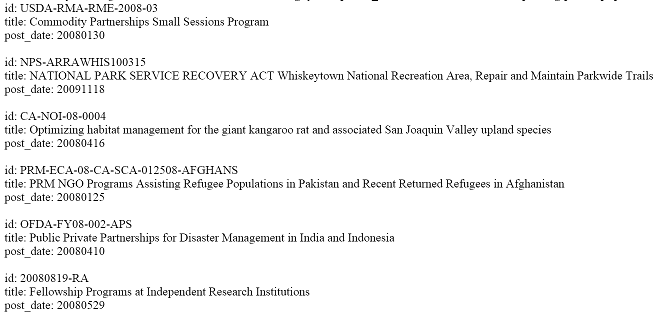
\includegraphics[width=0.8\textwidth]{senior_design_grants_output.png}
    \caption{Output from the Grants.gov parser}
    \label{fig:grants_output}
\end{figure}

\begin{figure}
    \centering
    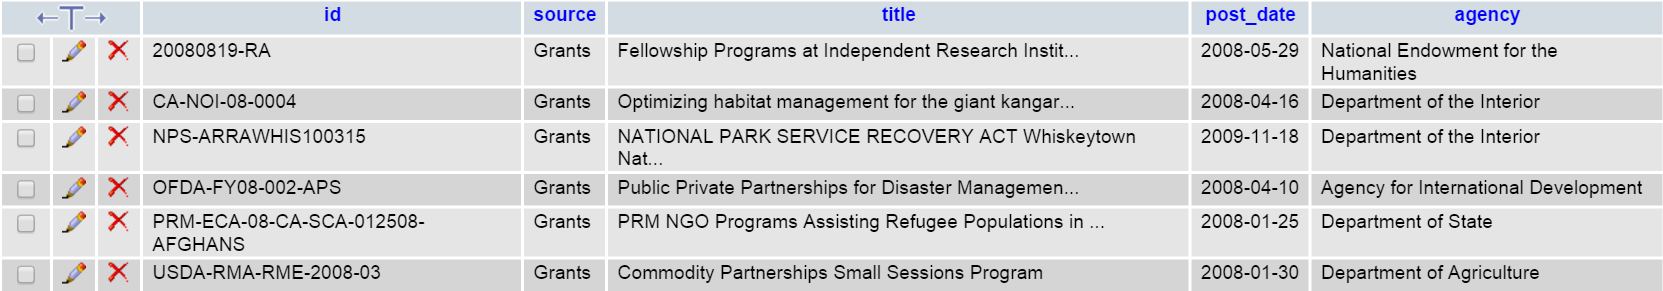
\includegraphics[width=0.8\textwidth]{senior_design_grants_db.png}
    \caption{Result of the Grants.gov parser}
    \label{fig:grants_db}
\end{figure}

\subsection{FedBizOpps Parsers}
We had a rough time implementing the parsers for the FedBizOpps files. As mentioned above, the FedBizOpps nightly file is not an XML file. For each funding opportunity, there is an element in the nightly file that has an opening TYPE and closing /TYPE tag. But the fields inside that element do not have closing /FIELD tags. So our parser needed to read through each line and construct the fields before adding them to the final SQL query. Due to the strange format of the nightly files, they cannot be parsed with XML parsing libraries. These files are essentially formatted text files. We were not able to figure to why the files were formatted this way instead of as actual XML files, or what user would prefer this format.  

Another confusing feature of the nightly files is that they contain HTML tags, as well as typical newlines. We were forced to decide whether to remove these tags ourselves, or allow them to stay in place. Ultimately we decided to remove most of the tags that might appear, because we do not want to allow opportunity descriptions to change our site format. 

The FedBizOpps weekly XML is more straightforward. It is proper XML and can therefore be parsed easily with PHP's existing XML parsing libraries. One of the more difficult problems in parsing the weekly file is that when an opportunity is amended or modified, the original record is not changed. Instead, all of the modifications are listed as records attached to the one that was modified. This requires the parser to check for modifications and iterate through them. Then, the record we want to store in our database must be updated sequentially until there are no more modifications.

Here is an example of the FedBizOpps weekly parser. It is much easier to find fields for each element by using the \$node variable.
\begin{Verbatim}[commandchars=\\\{\}]
\PY{x}{while(\PYZdl{}xml->read())}
\PY{x}{\PYZob{}}
\PY{x}{    // Read each element, skipping any that aren't interesting}
\PY{x}{    if(!(\PYZdl{}xml->nodeType == XMLReader::ELEMENT)}
\PY{x}{    || (!in\PYZus{}array(\PYZdl{}xml->name, \PYZdl{}types)))}
\PY{x}{        continue;}

\PY{x}{    // echo "}\PY{x}{<}\PY{x}{br>}\PY{x}{<}\PY{x}{br>&nbsp;&nbsp;&nbsp;" . \PYZdl{}xml->name . '}\PY{x}{<}\PY{x}{br>';}
\PY{x}{    \PYZdl{}node = new SimpleXMLElement(\PYZdl{}xml->readOuterXML());}

\PY{x}{    echo "NOTICE TYPE: " . clean\PYZus{}string(\PYZdl{}xml->name, \PYZdl{}mysqli) . ". SOLNBR: "}
\PY{x}{    . \PYZdl{}node->SOLNBR . "}\PY{x}{<}\PY{x}{br>";}
\PY{x}{...}
\end{Verbatim}


By contrast, here is an excerpt from the nightly parser. Because of the strange document format, each line read must be compared to a field identifier. We do not know when one field ends; we only know when the next begins.
\begin{Verbatim}[commandchars=\\\{\}]
\PY{x}{            // Try to find all elements that matter to our database}
\PY{x}{            if(strncmp(\PYZdl{}line, "}\PY{x}{<}\PY{x}{DATE>", strlen("}\PY{x}{<}\PY{x}{DATE>")) == 0)}
\PY{x}{                \PYZdl{}date = \PYZdl{}mysqli->escape\PYZus{}string(str\PYZus{}replace("}\PY{x}{<}\PY{x}{DATE>", "", \PYZdl{}line));}
\PY{x}{            if(strncmp(\PYZdl{}line, "}\PY{x}{<}\PY{x}{YEAR>", strlen("}\PY{x}{<}\PY{x}{YEAR>")) == 0)}
\PY{x}{                \PYZdl{}year = \PYZdl{}mysqli->escape\PYZus{}string(str\PYZus{}replace("}\PY{x}{<}\PY{x}{YEAR>", "", \PYZdl{}line));}
\PY{x}{            if(strncmp(\PYZdl{}line, "}\PY{x}{<}\PY{x}{AGENCY>", strlen("}\PY{x}{<}\PY{x}{AGENCY>")) == 0)}
\PY{x}{                \PYZdl{}agency = \PYZdl{}mysqli->escape\PYZus{}string(str\PYZus{}replace("}\PY{x}{<}\PY{x}{AGENCY>", "", \PYZdl{}line));}
\end{Verbatim}


While writing the FedBizOpps parsers, we noticed some peculiarities of the opportunity data that does not match their documentation. The date format that FedBizOpps uses needs to be transformed for SQL to understand it, but sometimes the date isn't actually a date; it's a classification code. We do not know why, but we believe it may be caused by agencies who have made an error in submitting an opportunity. Whatever the cause is, there is nothing we can do about it, because the error is in the XML itself. And although the FedBizOpps documentation states that certain fields are required to be non-null, those fields, in fact, be null. Another funny irregularity is that the titles in the XML are sometimes truncated, leading to interesting titles like '16--COUPLING,DRIVE SHAF,' where SHAF was probably supposed to be SHAFT. Again, these problems are in the FedBizOpps XML itself. Anyone can download the XML files and see for themselves. 

Early on in our project, there was some question about whether we should parse both files. If we parse only the weekly files, it would be easier to populate our database, and the data in it would not be out of data for long before updating. However, if we relied on the weekly files alone, our database would be out-of-date the day after parsing the weekly file. So we wrote the nightly parser to ensure our users only need to consult Connected to Research, and don't need to cross-reference with FedBizOpps to see if any opportunities have been modified or added.

\subsection{Database Description}
In the previous quarter, we developed a database design that we thought would allow us to implement our project in a timely manner. The entity relationship diagram we developed consists of five tables. The most important table is for our general funding opportunity information. It includes fields that we expect to be common and necessary for all funding opportunities, and is named ctr\_funding\_base. There are another two tables derived from this table, each for a specific funding source. One table is for Grants.gov funding opportunities. Another table is for FedBizOpps.gov funding opportunities. The generalized table holds the primary key which links to both Grants.gov and FedBizOpps.gov tables. 

Aside from the funding opportunities, there is a user table that includes user information such as phone number and email address. This table was already created by the previous team, but we needed to update it to add a list of interests. The last table is the interest table which compiles all of the categories and interests of the funding opportunities and users. The interests table maps a user's high-level description of their interests to a lower-lever code, such as an NAICS code.

Our funding sources assign each opportunity a value that marks it for some interested parties. FedBizOpps has NAICS codes. For example, an NAICS code that begins with 11 pertains to agriculture, forestry, fishing and hunting. Grants.gov uses eligibility categories, used similarly. We believe that users will not want to decode all of these cryptic identifiers when looking for funding, so our application will allow users to list interest descriptors in their user profiles. These descriptors will be stored in the user table under the 'interests' field. It will contain values along the lines of 'Toxicology, Chemistry, Herbology.' These interests will be connected to a category of interests in the ctr\_interests table, which will contain an array of all the NAICS codes, classification codes, and eligibility categories.

What we implemented is essentially identical to our data design of the database. The FedBizOpps.gov table consists of five columns and is named ctr\_funding\_fbo. These columns are sol\_number, notice\_type, award\_amount, award\_date, and set\_aside. The sol\_number is the key that will be linked to a primary key in the generalized table of funding opportunities. The sol\_number column's type is a varchar of 128 characters. A string variable type of 128 character is necessary because many of the sol\_numbers within the FedBizOpps weekly and nightly files have long names. 128 characters is the limit imposed by the FedBizOpps documentation, but the Grants.gov limit is much shorter. The notice\_type column is just a type of notice used by the agency offering the funding opportunity. This column's type is a varchar of eight characters because they are from a specific set of short strings. The award\_amount column holds the amount of money awarded for the opportunity. This column's type is a varchar of 64 characters. The award\_date column holds the date when the award was awarded. This column is a date type. The last column is set\_aside which holds the category of applicants that will be considered for the award. An example value is "women-owned small business." This column's type is a varchar of 60 characters, because these are also taken from a specific set of short strings.

The grants.gov table consists of 11 columns and is named ctr\_funding\_grants. These columns are opp\_number, \\
due\_date\_explanation, funding\_total, award\_ceiling, award\_floor, category\_explanation, instrument\_type, award\_number, elegibility\_category, eligibility\_info, and cost\_sharing.  The length of the columns is limited by the Grants.gov documentation. The opp\_number is the key that will be linked to a primary key in the generalized table of funding opportunities. The opp\_number column's type is a varchar of 40 characters. This is the maximum allowed by the documentation. The due\_date\_explanation column is a short description of the due date and time of which the application for the funding opportunities is due. This column's type is varchar of 255 characters as the descriptions can be long. The funding\_total column is the total amount of funding the agency is offering for the funding opportunity. This column's type is a varchar of 15 characters. The award\_ceiling and award\_floor columns are the greatest and lowest amounts offered to an individual for the funding opportunity. Both of these columns are of type varchar of 15 characters. The category\_explanation column is a description of all categories for the funding opportunity. This column's type is text since this element within the XML file of Grants.gov is one of the longest. The documentation limits it to 2500 characters. The instrument\_type column is just the instrument type of the funding opportunity. This column is of type varchar of two characters because this element within the XML file of Grants.gov contains one or two capitalized characters used as an abbreviation for an instrument type. The award\_number column is the amount of awards offered for the funding opportunity. This column's type is a varchar of 15 characters. The elegibility\_category column is a column that lists departments or interests categories. This column is the same column that would be inserted into the generalized table of funding opportunities as interests. This column is a char of two character because of the same reason as instrument\_type. The eligibility\_info column is a description of eligible applicants. This column is of type text due to being one of the longer strings. The cost\_sharing column is a column with a value of yes or no with the value 'Y' and 'N' respectively. This column describes if there is cost sharing or not and its type is of char of one character since it just holds the characters 'Y' or 'N'.

The generalized table of funding opportunities consists of 12 columns and is named ctr\_funding\_base. These columns are id, source, title, post\_date, due\_date, interests, agency, address, contact, office, url, and description. The size limits for these columns are taken from the upper bounds listed in the documentation from both Grants.gov and FedBizOpps. The id column is a primary key column that links with the FedBizOpps.gov and Grants.gov sol\_number and opp\_number columns respectively. This column is of type varchar of 128 characters. The source column is to specify where the funding opportunity originated from. Currently it is either 'Grants' or 'FedBizOpps'. This column's type is a varchar of 255 characters, because we may support more sources in the future. The title column is for the title of the funding opportunity. This column is of type varchar of 255 characters. The post\_date and due\_date columns are the date the opportunity was posted, and the date applications are due. They are both date types. The interests column list all of the interests or categories of the funding opportunity. This column is of type varchar of 255 characters. The agency column lists the agency that is offering the funding opportunity. This column is of type varchar of 255 characters. The address column contains the address of the agency. This column is of type varchar of 255 characters. The contact column contains the contact information which could include websites, email, and phone numbers. This column's type is of varchar of 300 character. The office column typically contains the name of the office of the agency, but at times contains the type of agency. This column is of type varchar of 255 characters. The url column contains the URL to the agency's website, application, or sometimes contains nothing. This column is of type varchar of 255 characters. The description column is most commonly the longest column, and contains the description of the funding opportunity. This column is of type text due to its length.
 
The user table consists of seven columns and is named ctr\_user. These columns are email, name\_f, name\_l, password, user\_img\_src, user\_occ, and interests. All columns are of type varchar of 255 characters. The email column contains the email of the user which is also used as a username. The name\_f column contains the first name of the user. The name\_l column contains the last name of the user. The password column contains the password of the user. The user\_img\_src column contains the image of the user. The user\_occ column contains the occupation of the user. The interest column contains the interests of the user. The user is able to have up to five interests. 
 
The interests table is named ctr\_interests. It has two columns, interests and category. Category is a descriptions that users are allowed to use in their list of interests. Interests is a list of all of the NAICS code and other values that may apply to that category. The interests are stored as an array encoded in text form, as a varchar of length 255. Each type of code is separated by semicolons and the values within are separated by commas. For example, an interests value of "cc:16;naics:61,55" will mean that the classification code is 16, and the NAICS codes are 61 and 55. Any opportunities that have these interest codes applied to them should be matched to a user whose table's interests column include the matching category string. 

And finally, we have several tables that need to be adapted from the previous team's implementation. We will essentially need to duplicate the ctr\_user\_fav and ctr\_user\_call\_link tables to implement our 'dog-ear' and bookmarking requirements. These were explained above, but the dog-ear feature will add the opportunity to a list for later review. Bookmarking will add it to a pane on the left which lists opportunities and their due dates. 

\subsection{Website Description}
The website currently displays three columns, each with a designated role. The left-most column acts as a sort-by filter, where the user may select which funding opportunities he or she would like to view. In the middle column is the main view of the funding opportunities, whose display is based on the left-side column filter. Lastly, the right-most column is planned to be a collection of the research events and deadlines currently and upcoming. All of these are contained in the funding.html file. Figure \ref{fig:filter} shows the filter on the left of the page, and an opportunity on the right. The top of the image shows the navbar, with the logged-in user's name and profile picture. 

\begin{figure}
    \centering
    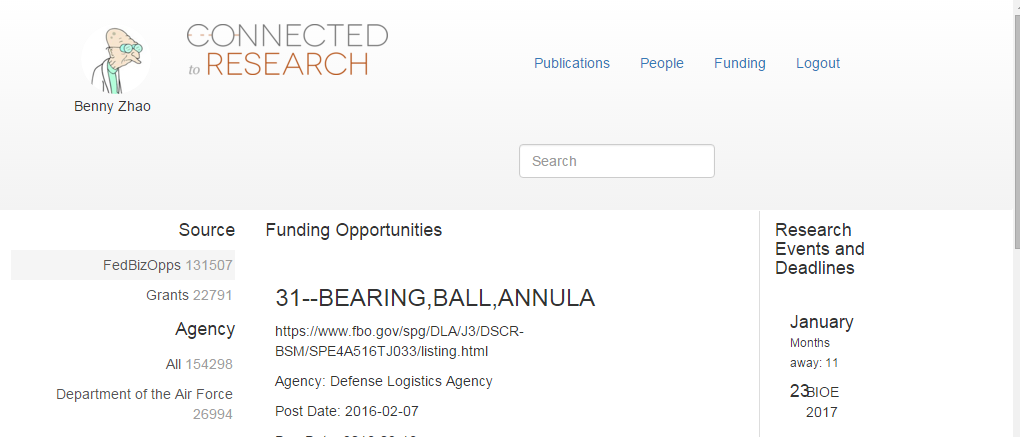
\includegraphics[width=0.8\textwidth]{filter.png}
    \caption{The funding page, showing filter and an opportunity}
    \label{fig:filter}
\end{figure}

Next we have a funding.js file that basically acts as a link between the Ajax PHP scripts and tpl.html files. Within the funding.js file are AngularJS directives and controllers that manipulate what the user views in funding.html. The directives that are currently in the JavaScript file are for the navigation bar, the filtering column, the funding item column, and the deadlines column. The directives are for creating custom html tags that can grab information from the .tpl.html files. Then we have the AngularJS controllers that holds JavaScript functions and grabs functionality from the Ajax PHP files in the Ajax directory. 

The controllers we currently have are the navigation bar controller and the funding controller. The navigation controller's role is to get the SQL query from the user-nav-bar-info.php and use the navigation bar directive tpl.html file to display the image of the user, first name and last name, and buttons that link to the other pages. Another controller that we have is funding controller that has majority of the JavaScript functions for the web application. In the funding controller, you can find a function for the filter column that calls the php script filter-funding.php. This allows the filter column to display filtering criteria based on the SQL queries in the filter-funding.php file. Within the filter-funding.php are PHP prepared statements that executes the SQL queries and then after the prepared statements are executed the results are returned to an array of arrays in the same file. The array of arrays maps key-value pairs that are returned to the filter-funding.tpl.html file and then to the user view. 

Another function inside the funding controller is the function for calling the funding item in the main view. The role of this function is to get the results from funding-items.php based on the parameter type the user selects from the filter column. Then it displays all the relevant funding opportunities in the main funding column to the user. The last function that is in the funding controller is targeted for the deadlines column where it grabs the results from the funding deadlines PHP file. This happens when the user wants to bookmark a funding opportunity, so they can be reminded of the due dates and time ranges. 

\subsection{Necessary Adaptations}
Our interface was designed before we started our project. We did not have to meet with our client to get their opinions on it. We have mockups created by the previous team, who likely created the mockups themselves with actual HTML and JavaScript. But we've needed to adapt some of the previous team's work to make our component work. The previous team used JavaScript functionality and templates that were specific to their own component. To bring our own work into the site's design, we needed to adapt their work to make ours have its own distinct look. For the most part, we have had to duplicate their code and make minor changes to it to make it specific to the funding component information. As an example, we needed to add functionality for the filter bar on the right side of the page. To do so, we could not use the previous team's filter bar PHP script. Instead, we needed to create our own that was roughly similar, but allowed for dynamic filter types. The previous team used statically defined filters but our client asked us to allow users to filter based on the agencies in our database, which requires us to list the agencies in the filter bar.

We also need to modify their templates. Our templates are mostly the same, but need to support more functionality. In the filter example, we used the same template as the previous team. Only the PHP script that created the data for the filter panel needed to be changed. As for the actual funding items, we will need to create our own template. According to the designs that the previous team developed with the client, the previous team's template does not include enough data to satisfy our client's designs. At the same time, we cannot match their mockups exactly. Their mockups list the funding opportunity dollar amount, but that data is not available for most opportunities. They also list different types of due dates, but only one general due date is available from both of our funding sources. We do not have a way to check the 'concept paper due date' or the 'proposal due' date. Instead, we will need to limit the fields that are displayed to what will provide the most context for the opportunity with our data. Figure \ref{fig:mockup} shows the prvious team's mockup. It can be compared to figure \ref{fig:filter}, but our implementation is sort of a stand-in at the moment.

\begin{figure}
    \centering
    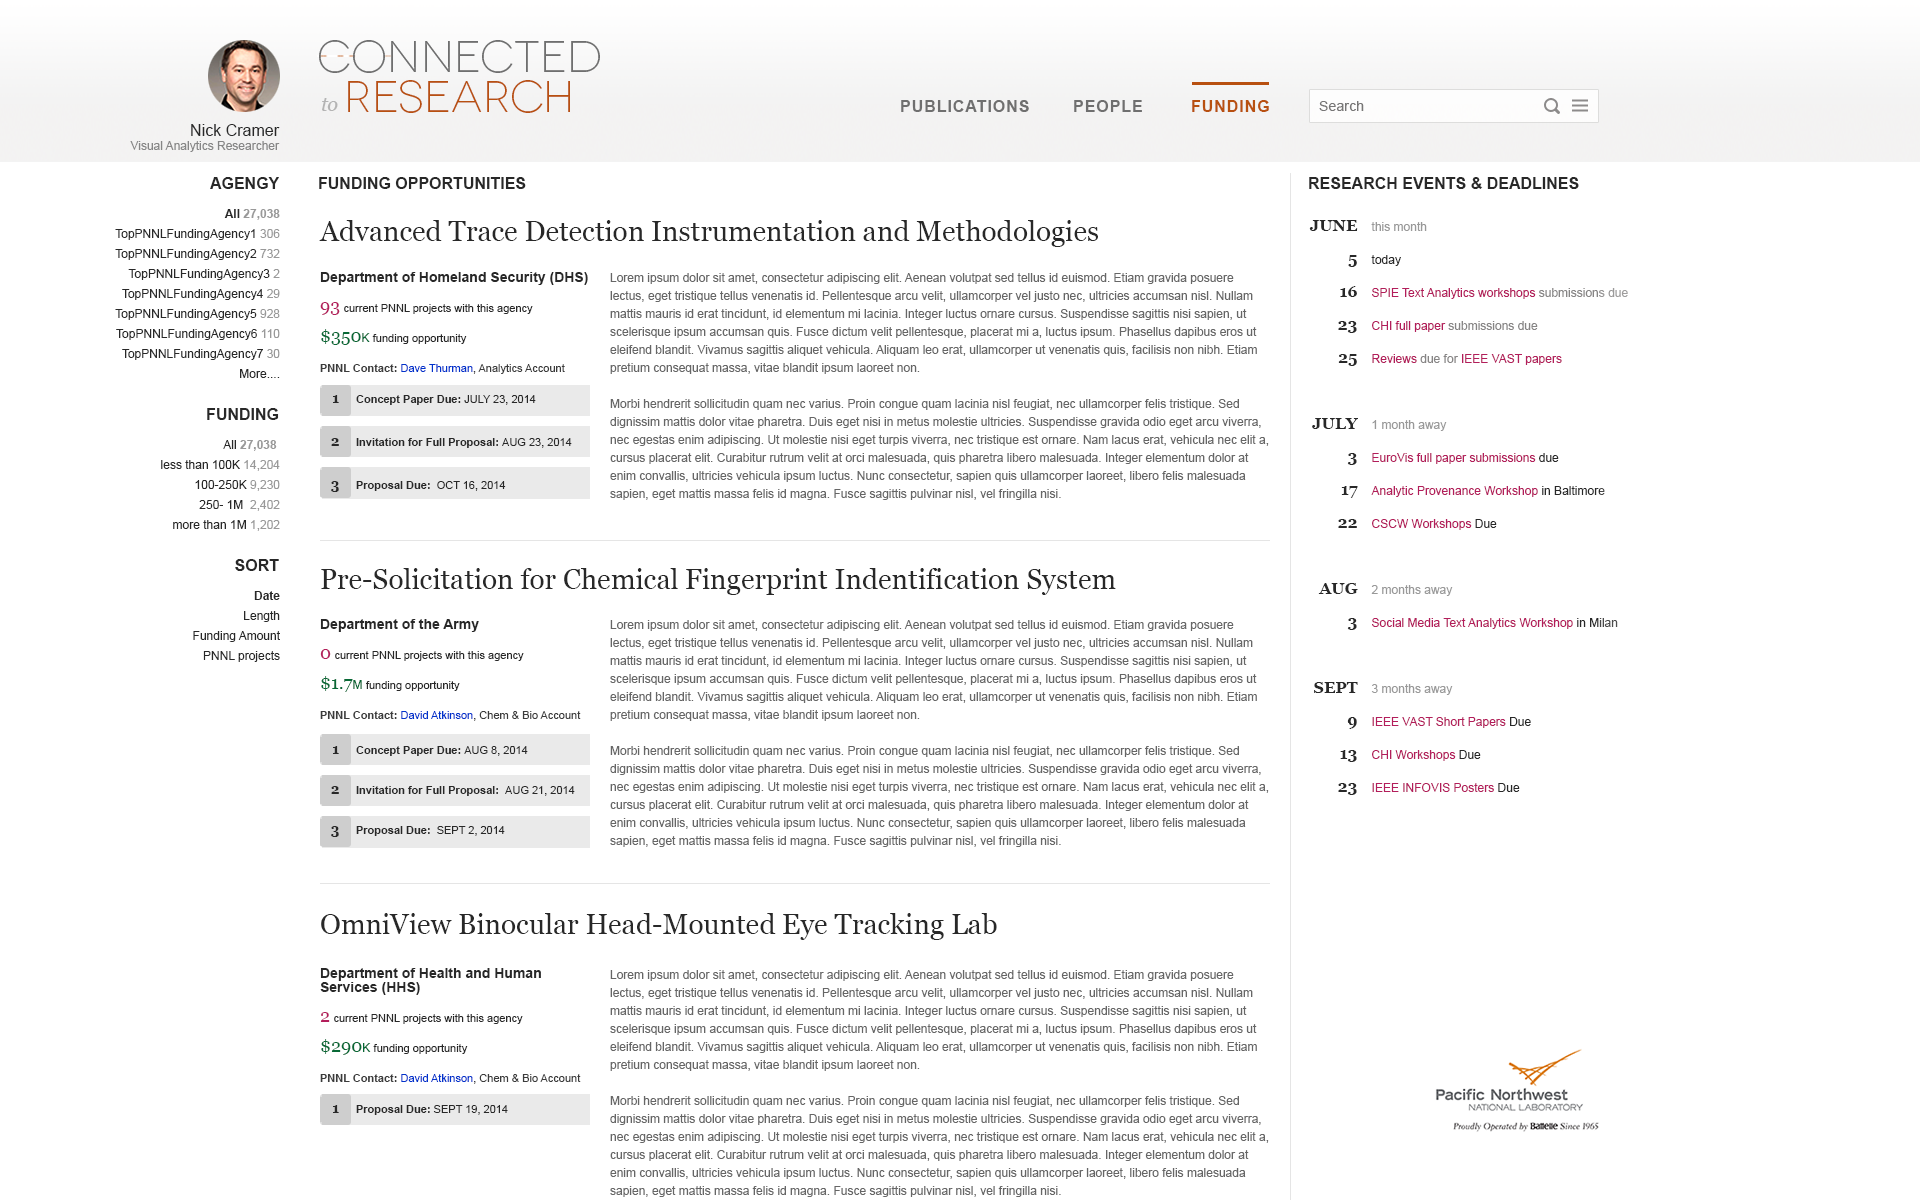
\includegraphics[width=1.0\textwidth]{funding-default-view.png}
    \caption{Example from the previous team's mockup}
    \label{fig:mockup}
\end{figure}

\subsection{Client Meetings}

At the start of this term, our client decided that they would like to have bi-weekly meetings with our group. The first meeting we had was on January 11\textsuperscript{th},  where our client wanted to discuss the deliverables that our group is required to complete for this quarter and any questions we may have pertaining to the project. During the meeting, we discussed about the upcoming deliverable deadlines and how to best plan for them.

During the second meeting that happened on January 25th, we discussed our current progress on the project, questions to clarify the design of the interface, and goals that still need to be reached. In the meeting, we explained how our parser works to our client and what we have so far on planning the interface design. The client informed us that they wanted a funding webpage that is able to sort the funding opportunities based on certain filter criteria. They also gave us general criteria of what filters we should create for the UI based on what our parser inputs into our database. What the client would like on the display of the website has definitely changed due to some constraints of what information we can grab from either Grants.gov or FedBizOpps. 

Our client wanted us to create a filter for the funding opportunities which will split the view into three parts. One part is the left side where all of the filter buttons will be located, the center where it will display the funding opportunities based on the filter, and the right side where all of the funding opportunities' deadlines will be located. 

In order to implement the filter, we had to create a similar design to the previous team in order to keep the design consistent. At first there was a challenge in making the filter display itself. But as we went through the code, we found there to be typos and one of the typos was the bug to why we could not see our filter. Once we got the filter column to show up. We had to implement the SQL queries step-by-step because if a SQL query didn't work properly, we would not be able to see our output. After we got a framework of the filter column, we needed to make it more tailored to what the user would want to see. Therefore we used nested arrays within our filter in order to be as detail as possible so that the user doesn't have to spend much time scrolling through the funding opportunities.

%%%%%%%%%%%%%%%%%%%%%%%%%%%%%%%%%%%%%%%%%%%%%%%%%%%%%%%%%%%%%%%%%%%%%%%%%%%%%%%%
%%%%% WORK TO BE DONE
%%%%%%%%%%%%%%%%%%%%%%%%%%%%%%%%%%%%%%%%%%%%%%%%%%%%%%%%%%%%%%%%%%%%%%%%%%%%%%%%
\section{Work To Be Done}
Currently, our databases don't involve the user interests. Each funding opportunity has categories applied to it. For example, FedBizOpps has NAICS codes and classification codes. Users will not want to specify a long list of NAICS codes that they are interested in, so our app will allow them to list a high-level description, such as 'toxicology'. The high-level descriptions are matched to the low-level codes using the interests table. In the future, we will need to add functionality to the script that populates the main funding page. It will need to get the interests of the user currently logged in and perform an extra query to select only the funding opportunities that the user might be interested in. Currently, we are simply showing 10 of the most recent opportunities posted, after applying a filter.

Once we have finished the functionality for the user interests, our project is mostly complete. The 'sharing' feature listed in our requirements document was already completed by the previous team. We only need to expand it so that users can email opportunities to other users. This will be relatively simple using JavaScript. We only need to add a 'mailto' link to the pop-up share menu the previous team implemented.

We also need to implement a bookmarking system. This, as well, will only need to be adapted from the previous team's work. They have the 'events and deadlines' panel working, with a table in the database to list research opportunities. We will need to modify the database table to store research opportunities that the user has bookmarked. Then, we need to add more logic to the script that populates the deadlines panel.

We will need to support 'dog-ear'-ring opportunities for later review. This was also implemented for the publications component. The bookmarking feature is mostly the same. Both will need to have their own database tables. The bookmarked opportunities will be used to populate the deadlines panel. The dog-eared opportunities will need to have their own place to be displayed. We have not decided this with the client, but we are currently considering two options. For one, we could create a user page, and create a 'dog-ear' subpage. The dog-eared opportunities can be listed there. Alternatively, we could list the dog-eared opportunities on the funding page, in their own marked section at the top of the list of opportunities. With the first approach, users might just forget about the opportunities. With the second, they might get annoyed at having to scroll past them every time they load the page. We may have to implement mockups of both to see which the users prefer.

\section{Problems We've Encountered}
One of the conflicts that we came by was the creation of the filter column in funding.html. We tried to create a Javascript file that would create directives and controllers to bind to the funding.html webpage. The issue we tackled was trying to get the filter column to display based on what filter-funding.php queried, but there was a binding parameter error. So we took out the parameter binding, but the funding.html still didn't grab the necessary information, when the filter-funding.php script was already working. 

The Grants XML parser has a memory usage limit conflict. When working on Oregon State University's server, the memory usage limit for PHP is 68 megabytes. This is a conflict because the XML files that needs to be parse for the project is 128 megabytes or more. The problem lies within the program when a buffer gets the XML file. Whenever the buffer holds over 68 megabytes the program would return an error then the program would terminate. A potential solution is to grab each grant structure in the XML file individually then free the memory after inserting the opportunity into the database. By going grabbing each grant structure individually, the buffer would hold small amounts of data at every given time of the program's execution. Another problem with the Grants XML parser is that some of the elements in the Grants structure could either be a single string or an array of multiple strings. This was a problem because the database table accepts only a string. If an array was inserted then it would show up in the database as "Array" rather than its values. The solution to this was simple. Simply check if the element is an array and if it is then concatenate all of its members into a single string variable separated by commas.  Then insert the string into the database to its respective column.  

\end{document}
